\section{Data warehouse design}

The data warehouse stores all parsed information and creates OLAP-Cubes to achieve fast responses 
for even the most complex of queries.

\subsection{Schema}
The data may be stored in the following schema. If optional functions are implemented and
the warehouses are configured dynamically, the schema may diverge from this.
\begin{center}
%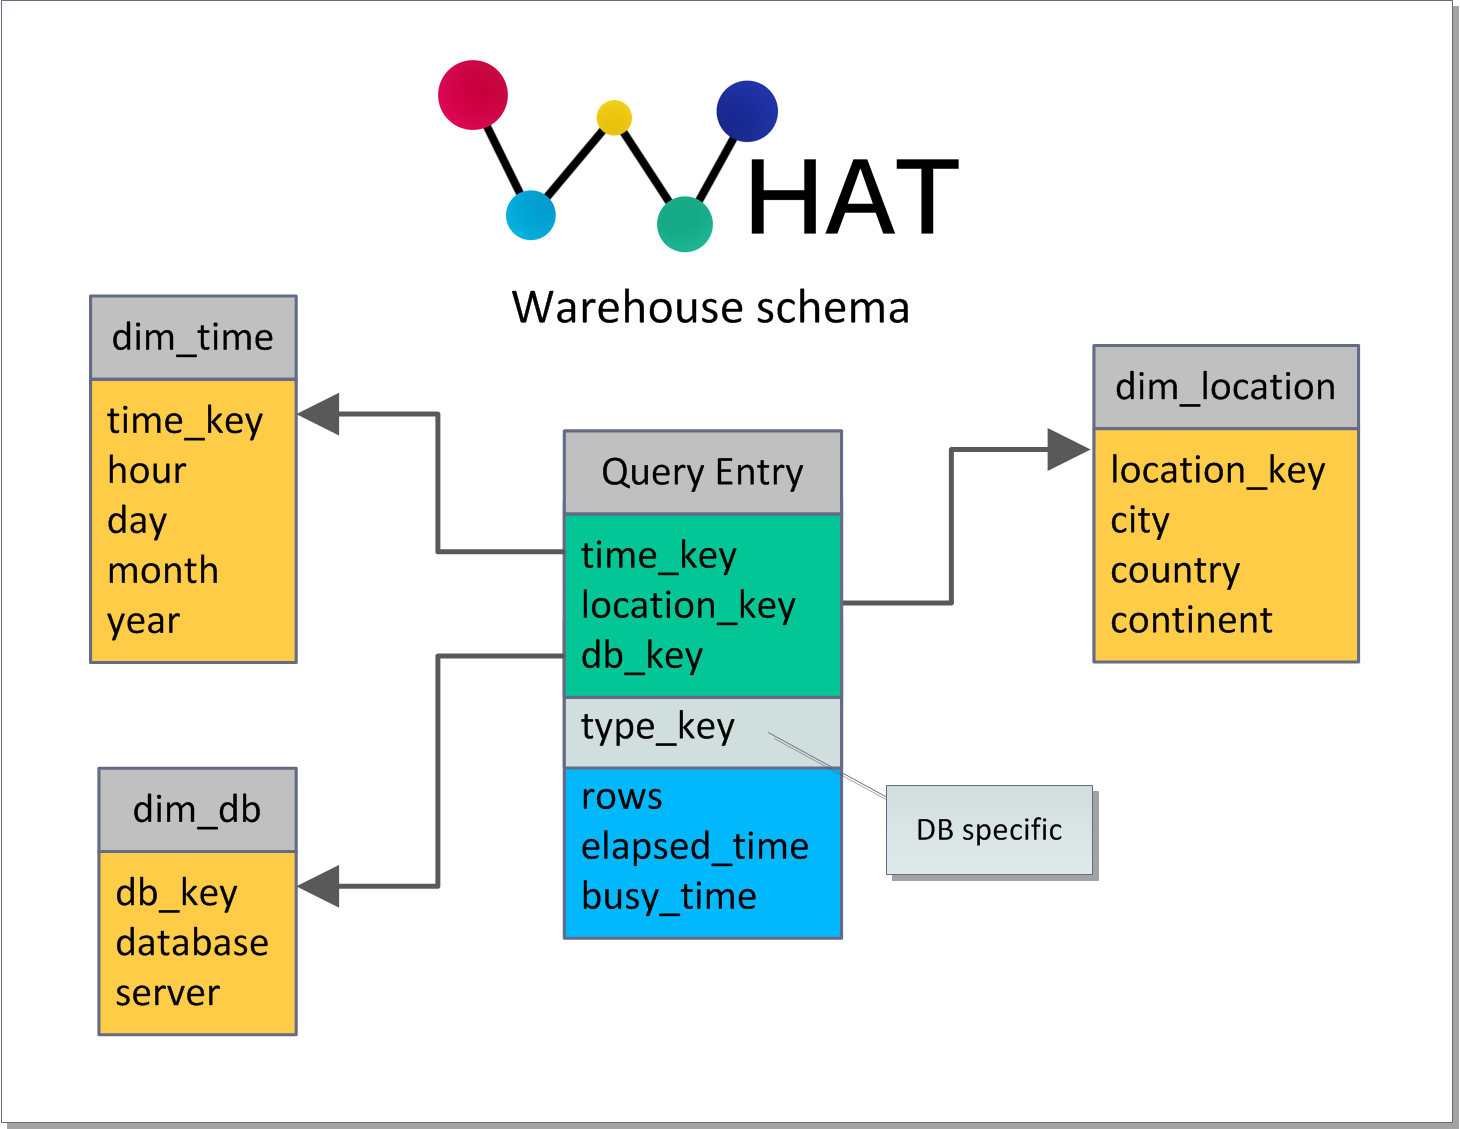
\includegraphics[width=1\linewidth]{Pictures/WHSchema.png}
% or
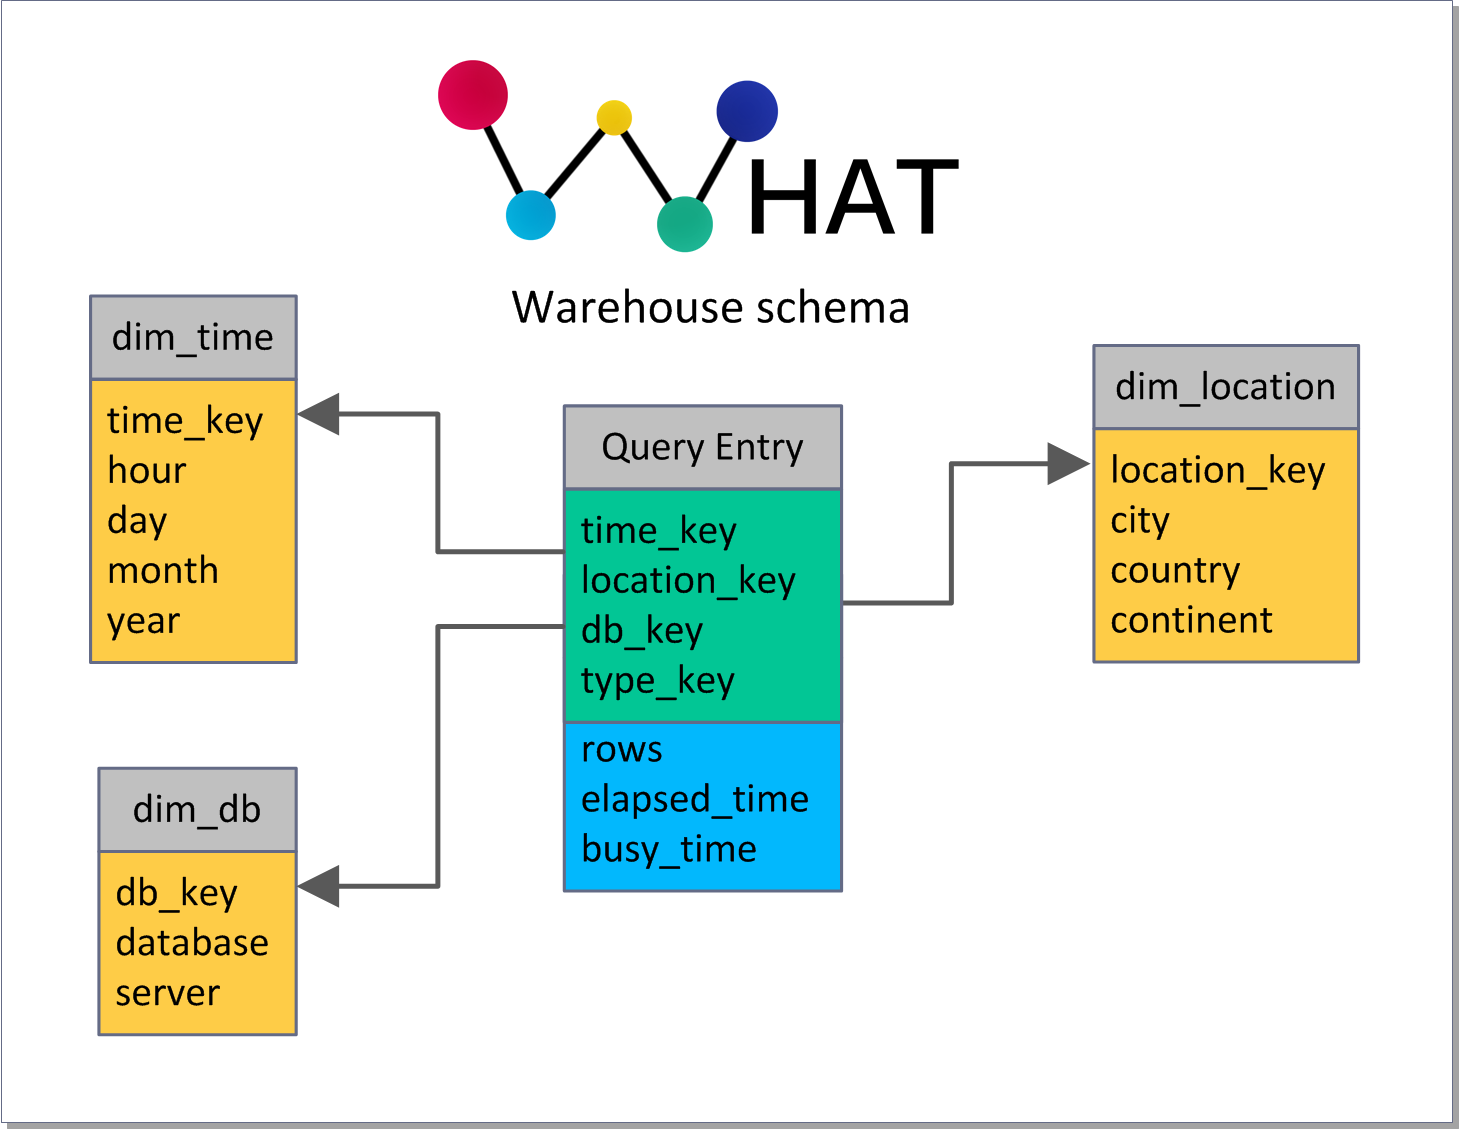
\includegraphics[width=1\linewidth]{Pictures/WHSchema2.png}
\end{center} 


\subsection{Dimension descriptions}
 The only database independent dimensions are time and location. The time dimension is defined by us. The location 
 dimension is given by the GeoIP-lib. (\ref{geo}).
 
 BILD TIME DIMENSION

Other dimensions like database > server, type and maybe others, 
depend on the database operated on, e.g. SkyServer.


\subsection{Measure descriptions}
Measures are for example busy time (CPU time), elapse time and rows. The aggregations stored in the
OLAP-Cubes for this measures are:
\begin{itemize}
 \item sum of their value,
 \item maximum of the value overall in all levels below,
 \item maximum of the values stored for sum in the level below,
 \item number of entries in a level below.
\end{itemize}



  
